% !TeX root = ../thuthesis-example.tex

\chapter{绪论}


%
\section{研究背景与意义}

近年来,人工智能技术的发展始终处在快车道,在全球范围内不断取得重大突破,逐渐成为引领性技术。
从统计分析到智能感知再到生成式AI和智能预测,以机器学习为首的人工智能技术持续在不同领域不同任务上发光发热,不断为各行各业带来革命性的转变。
世界各国和主要经济体纷纷加快人工智能战略布局,并相应出台了一系列人工智能发展规划、政策和法律法规。
美国的《国家人工智能研究与发展战略计划》、欧盟的《人工智能法案》、我国的《数字中国建设整体布局规划》和《全球人工智能治理倡议》等一系列战略文件,都明确了人工智能技术的重要性和发展方向,推动着产业界和学术界的技术创新和应用落地。

技术变革的阶段往往也是野蛮生长的阶段,人们关注的焦点大多是如何快速地深化技术,以搏取先发优势和领导者地位。
但当技术面临落地时,工程化、标准化、规模化等方面的诸多挑战开始凸显,制约着其应用推广。
对于机器学习而言,技术增长期常见的“烟囱式”、“手工作坊式”等不成体系的研发模式是造成其应用成本高、管理乱、落地难的重要原因:
一方面,模型研发的工作流程缺乏顶层设计,分工不明确,易出现重复劳动,难以形成有效的团队协作;
另一方面,模型研发过程中产生的资产缺乏统一的存储和管理,资产易流失,经验难传承,难以形成有效的知识沉淀和复用。
本文研究的意义正在于此,通过构建机器学习平台,以工程化的手段来解决这些问题。

\begin{figure}
  \centering
  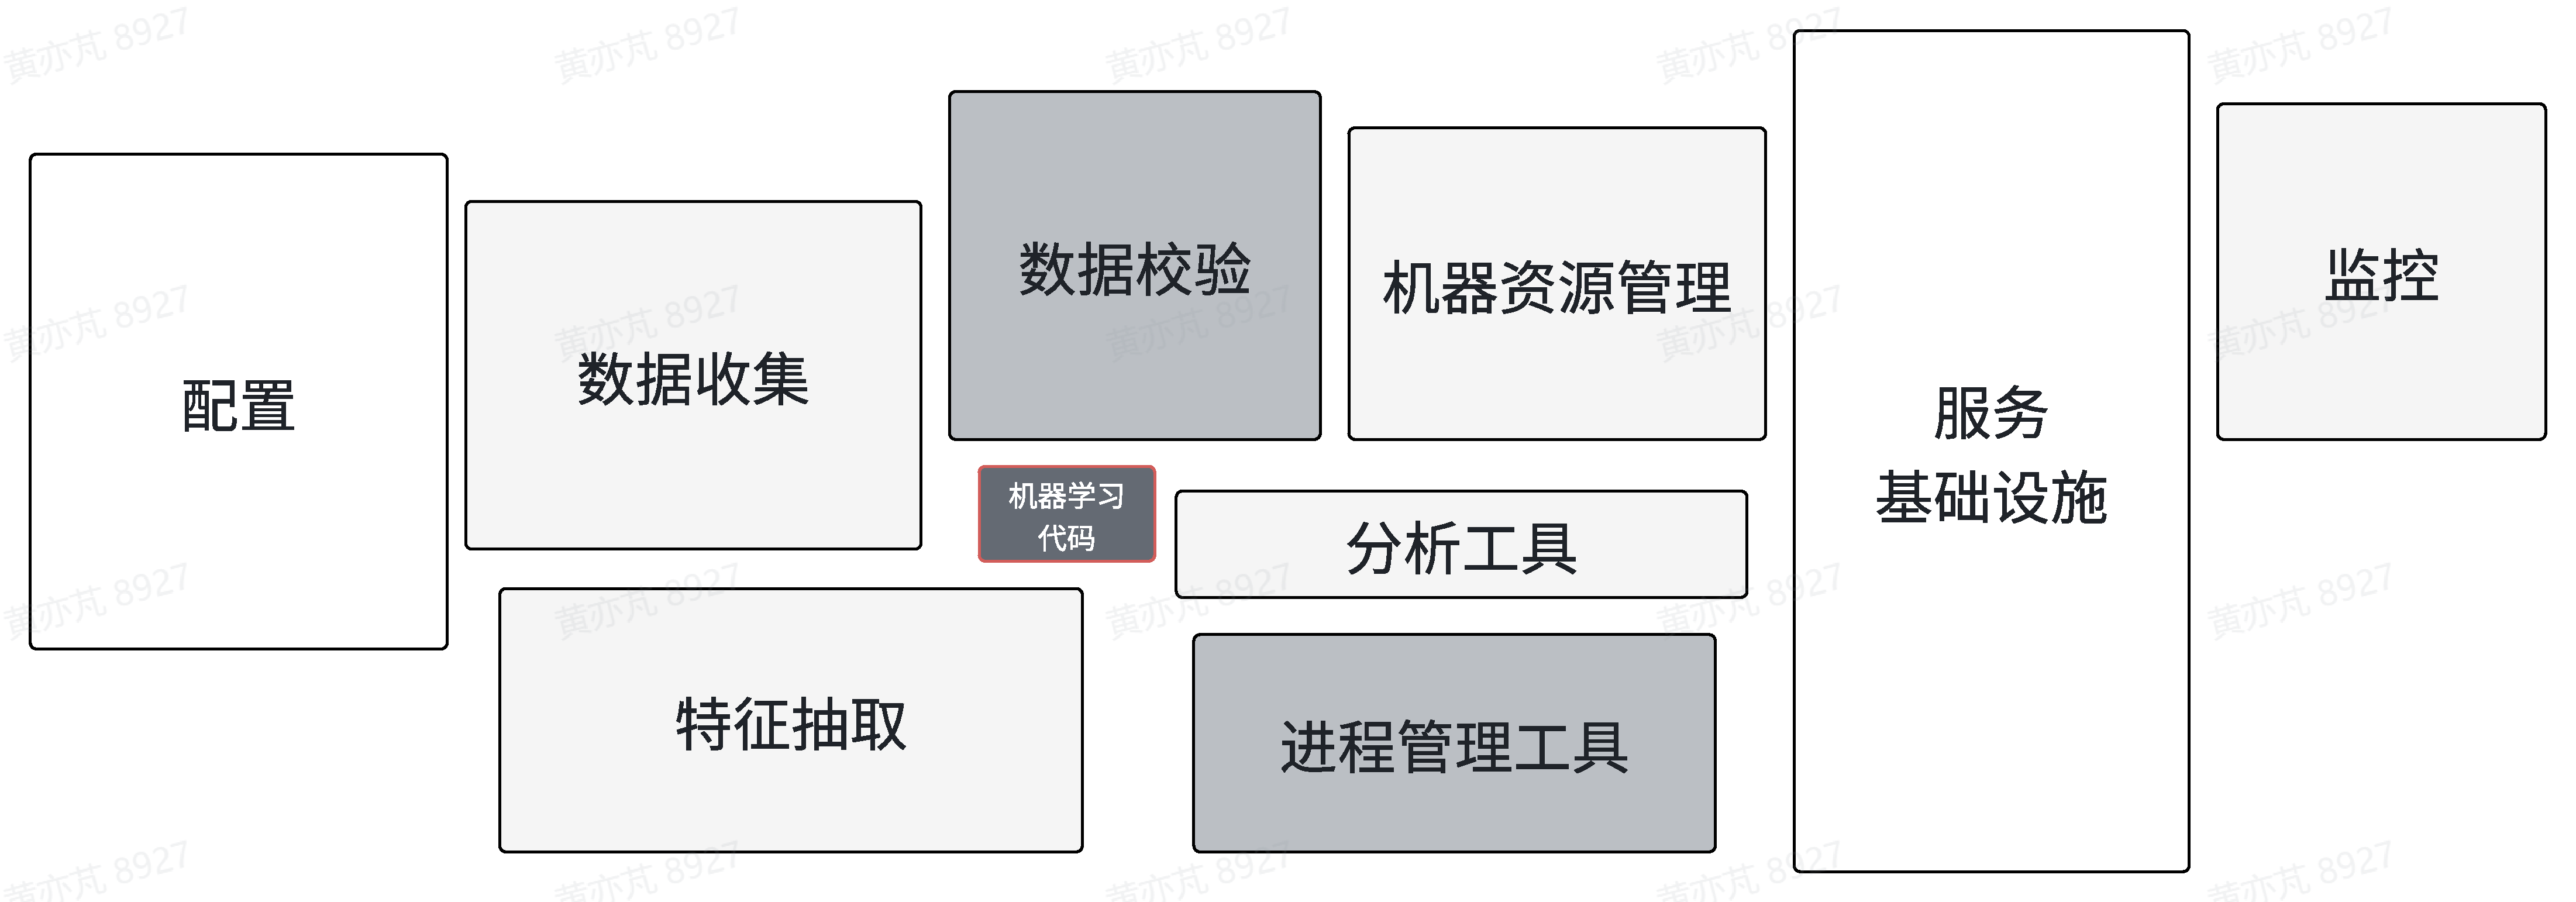
\includegraphics[width=0.98\linewidth]{ml-system-components.pdf}
  \caption{谷歌提出的机器学习系统组成}
  \label{fig:mlcomponents}
\end{figure}

人类的技术发展总是伴随着工程化的进程:从人力种植到机械耕作、从手工制造到工业生产、从编程开发到软件工程等等。
其中的关键是工具手段的出现和演进以及流程的标准化和自动化,以支撑技术的规模化应用。
其核心就是提高生产效率,从而解放生产力,降低生产成本,提高产品质量。
在机器学习领域,工程化的进程也是必然的,也是迫切的。
正如谷歌在机器学习系统设计的奠基性理论研究中所提出的,真实世界的机器学习系统中包含广阔而复杂的工程化基础设施,机器学习代码只是系统中很小的一部分,如图\ref{fig:mlcomponents}。
在模型核心技术研发的层面上,数据准备、算法开发、模型训练、模型评估等环节需要工具手段的辅助,以提高研发效率和模型性能;
在模型应用落地的层面上,模型部署、模型监控、流程自动化、业务应用集成等环节更需要工程化的系统软件支撑,以保证应用的稳定性、可靠性和可维护性。

【与软件工程的不同】
模型结构复杂、训练数据多、参数量大、随机性强

【为什么云原生】

需要注意的是,一些文献中将PyTorch、TensorFlow等机器学习计算框架称为机器学习平台,易与本文的研究对象混淆。
本文研究的机器学习平台是指支撑机器学习研发和应用的软件工具系统,依托于硬件基础设施(或称硬件平台,亦与本文中的平台不同),支持在平台中使用PyTorch、TensorFlow等机器学习计算框架进行模型训练、推理等计算作业。


%
\section{国内外研究现状}

TBD

\subsection{理论方法}

TBD

\subsection{工具系统}

TBD


%
\section{研究内容与主要贡献}

TBD


%
\section{本文结构安排}

TBD
